% Nounce V2 poster — A0 landscape, 4 columns.
% Build with tectonic (XeTeX): tectonic poster-v2.tex
% Figures resolve relative to doc/report/ (figures/, images/).
% This is a wired-up skeleton matching doc/poster-v2.md; tune spacing/sizes to taste.

\documentclass[25pt, a0paper, landscape, margin=12mm, innermargin=14mm,
               blockverticalspace=10mm, colspace=14mm, subcolspace=8mm]{tikzposter}

\usepackage{graphicx}
\usepackage{amsmath}
\usepackage{booktabs}
\usepackage{fontspec}
% IPA-capable font for phone glyphs (same fallback chain as the report).
\IfFontExistsTF{Charis SIL}{\newfontfamily\ipafont{Charis SIL}}{%
 \IfFontExistsTF{Doulos SIL}{\newfontfamily\ipafont{Doulos SIL}}{%
  \IfFontExistsTF{STIX Two Text}{\newfontfamily\ipafont{STIX Two Text}}{%
   \newfontfamily\ipafont{Arial Unicode MS}}}}
\newcommand{\ipa}[1]{{\ipafont #1}}

\graphicspath{{figures/}{images/}{images/screen/}}

% ---- Palette (canonical = red, perceived = blue), matching the report charts ----
\definecolor{nounceBlue}{HTML}{1E3A8A}
\definecolor{perceived}{HTML}{4F81BD}
\definecolor{canonical}{HTML}{C0504D}
\definecolor{accent}{HTML}{F97316}
\definecolor{ink}{HTML}{1F2937}

\definecolorstyle{NounceStyle}{}{
  \colorlet{titlefgcolor}{white}
  \colorlet{titlebgcolor}{nounceBlue}
  \colorlet{backgroundcolor}{white}
  \colorlet{framecolor}{nounceBlue}
  \colorlet{blocktitlebgcolor}{nounceBlue}
  \colorlet{blocktitlefgcolor}{white}
  \colorlet{blockbodybgcolor}{white}
  \colorlet{blockbodyfgcolor}{ink}
  \colorlet{notefgcolor}{ink}
  \colorlet{notebgcolor}{white}
}
\usetheme{Default}
\usecolorstyle{NounceStyle}
\usetitlestyle{Filled}
\useblockstyle{Default}

% ============================ Title ============================
\title{\parbox{0.92\linewidth}{\centering
  Nounce: Perceived-Label Fine-Tuning for\\ English Pronunciation Assessment\\[6mm]
  {\large\normalfont\itshape ``detecting what learners say --- not what the dictionary says''}}}
\author{Ümit Can Evleksiz \quad\textbar\quad Ömer Faruk Bayram}
\institute{Dept.\ of Computer Engineering, Boğaziçi University \quad\textbar\quad Advisors: Prof.\ Lale Akarun, Prof.\ Murat Saraçlar}

\begin{document}

\maketitle[width=0.98\textwidth, titletotopverticalspace=8mm,
           titletoblockverticalspace=14mm]

% =========================================================================
\begin{columns}

% ---------------- COLUMN 1 : Problem & the data gap ----------------
\column{0.25}

\block{1. Problem \& the Data Gap}{
  Turkish-native learners lack accessible, specific pronunciation feedback:
  \begin{itemize}
    \item \textbf{Limited access} to native speakers / quality instruction
    \item \textbf{Generic feedback} --- ``try again,'' no phonetic detail
  \end{itemize}
  \vspace{4mm}
  The deeper obstacle is technical: phonetic models like \textbf{POWSM} are
  trained on \textbf{canonical} (dictionary) transcriptions --- produced by
  \emph{automatic} IPA methods --- so they \emph{normalize away} the very errors a
  tutor must surface.
  \vspace{4mm}

  \textbf{The data gap:} almost no public corpus gives the \textcolor{perceived}{\textbf{perceived}}
  (produced) phone sequence for L2 English --- the one signal a deviation detector
  must learn from. We bridge it with \textbf{L2-ARCTIC} (canonical + perceived on
  identical audio) and a small expert-annotated Turkish set.
}

\block{Canonical vs.\ Perceived}{
  \begin{center}
  % TODO: recreate the V1 phone-vs-phoneme explainer here (not a repo asset).
  % Relabel dictionary form = canonical (red), realizations = perceived (blue).
  \fbox{\parbox[c][9cm][c]{0.86\linewidth}{\centering
    \textbf{[GRAPHIC: canonical vs.\ perceived]}\\[4mm]
    one \ipa{/wʌn/} (canonical)\\
    $\rightarrow$ \ipa{[wʌn]} \ipa{[wʌŋ]} \ipa{[wʌn̪]} (perceived)\\[3mm]
    {\small differing phones highlighted in \textcolor{canonical}{red}/\textcolor{perceived}{blue}}}}
  \end{center}
}

% ---------------- COLUMN 2 : System (V1 -> V2) ----------------
\column{0.25}

\block{2. System (V1 $\rightarrow$ V2)}{
  A reliable, deviation-aware pipeline. Browser $\rightarrow$ TanStack app
  $\rightarrow$ a \textbf{single} stateless RunPod serverless POWSM worker
  $\rightarrow$ per-phone feedback; Neon + R2 below.
  \vspace{4mm}
  \begin{center}
    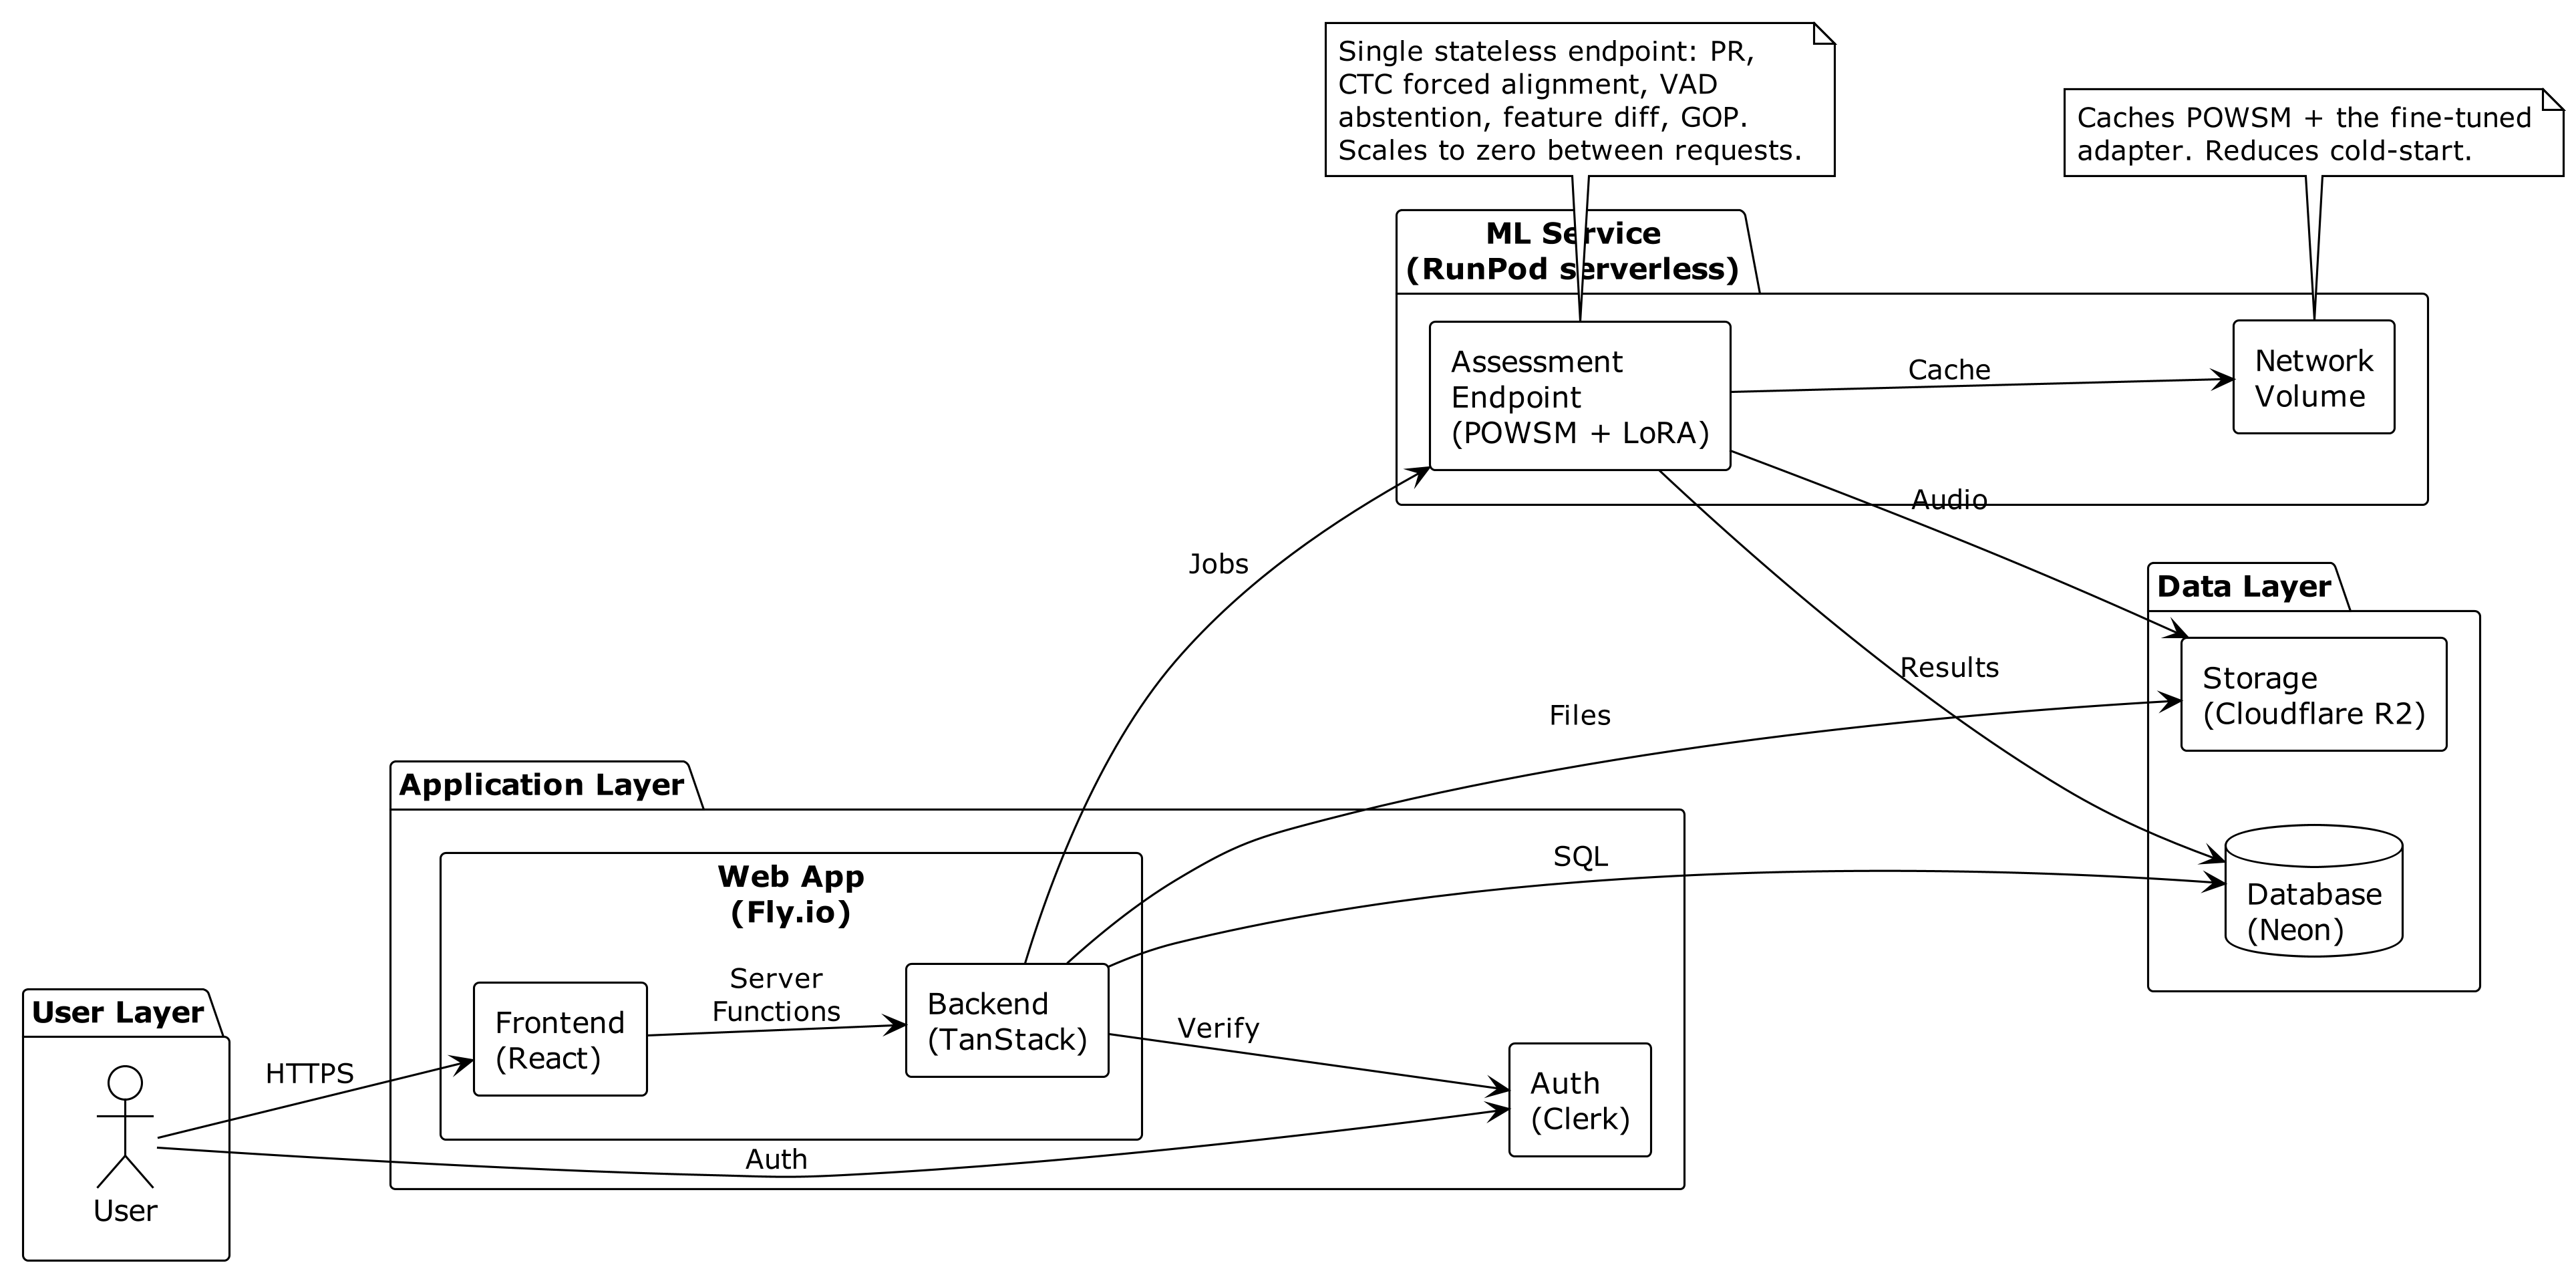
\includegraphics[width=0.96\linewidth]{deployment-architecture.png}
  \end{center}
}

\block{What changed since the prototype}{
  \renewcommand{\arraystretch}{1.35}
  \begin{tabular}{p{0.42\linewidth} p{0.5\linewidth}}
    \toprule
    \textbf{V1 prototype} & \textbf{V2} \\
    \midrule
    MFA for timestamps & POWSM CTC forced alignment (one model, one inventory) \\
    Two endpoints (G2P + PR) & One stateless worker \\
    Exact-match phone diff & PanPhon articulatory feature distance \\
    Scores any audio & Abstains on no-speech / noise / wrong sentence (VAD + SNR) \\
    Off-the-shelf POWSM & + Turkish-deviation-aware LoRA adapter (deployed) \\
    \bottomrule
  \end{tabular}
}

% ---------------- COLUMN 3 : The finding (centerpiece) ----------------
\column{0.25}

\block{3. The Finding}{
  A \textbf{controlled ablation}: same audio, same LoRA recipe ($r{=}32$,
  $\alpha{=}64$) --- only the \textbf{label target} changes.
  \begin{itemize}
    \item \textcolor{canonical}{\textbf{Canonical}} $\rightarrow$ recall drops
      \emph{below} baseline (\textbf{0.163 < 0.173}): \emph{actively harms}.
    \item \textcolor{perceived}{\textbf{Perceived}} $\rightarrow$ recall
      \textbf{0.213} + best Turkish PER (\textbf{0.392}).
    \item Gap \textbf{widens $\sim$4$\times$} from 30 to 60 epochs.
  \end{itemize}
  \vspace{3mm}
  \begin{center}
    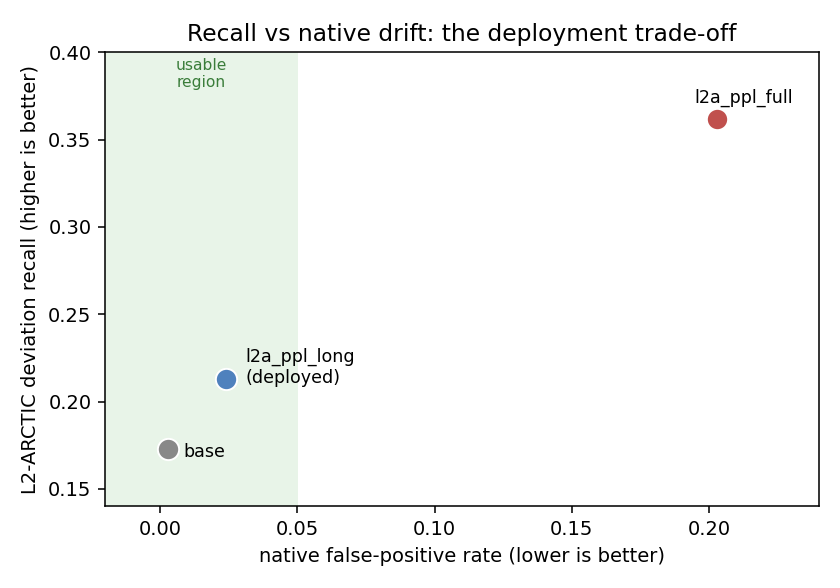
\includegraphics[width=0.96\linewidth]{recall_vs_fpr_frontier.png}\\[2mm]
    {\small Highest recall $\neq$ deployed: \texttt{l2a\_ppl\_full} flags 1-in-5
    correct native phones. We ship the conservative \texttt{l2a\_ppl\_long}.}
  \end{center}
  \vspace{2mm}
  \begin{center}
    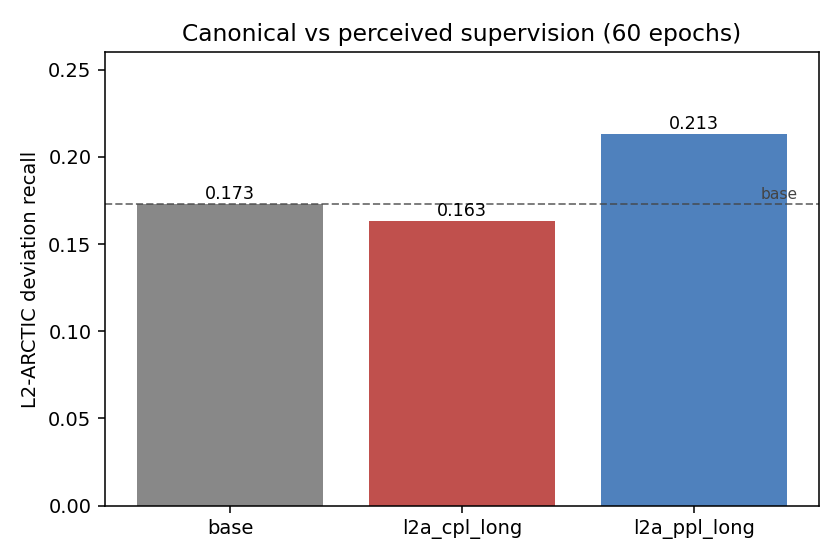
\includegraphics[width=0.7\linewidth]{l2arctic_cpl_vs_ppl_long.png}
  \end{center}
}

\colorlet{blocktitlebgcolor}{accent}
\colorlet{blockbodybgcolor}{accent!12}
\block{}{
  \centering\large
  \textbf{Convention beats quantity:} the label target decides whether
  fine-tuning builds a \emph{deviation detector} or just a better
  \emph{transcriber}.
}
\colorlet{blocktitlebgcolor}{nounceBlue}
\colorlet{blockbodybgcolor}{white}

% ---------------- COLUMN 4 : Validation & future work ----------------
\column{0.25}

\block{4. Validation}{
  \textbf{Human raters} (blind, 0--10 intelligibility): system vs.\ mean rating
  Spearman $\rho = \textbf{0.37}$ --- \emph{preliminary}: 2 raters, weak agreement
  (Krippendorff $\alpha = 0.11$); more raters is the bottleneck.
  \vspace{2mm}

  \textbf{speechocean762} (47k phones, Mandarin-L1): GOP rises monotonically with
  expert accuracy; $\rho = 0.21$ phone-level, \textbf{0.37 sentence-level} --- same
  $0.37$ as the human study. Generalizes to a different L1.
  \vspace{3mm}
  \begin{center}
    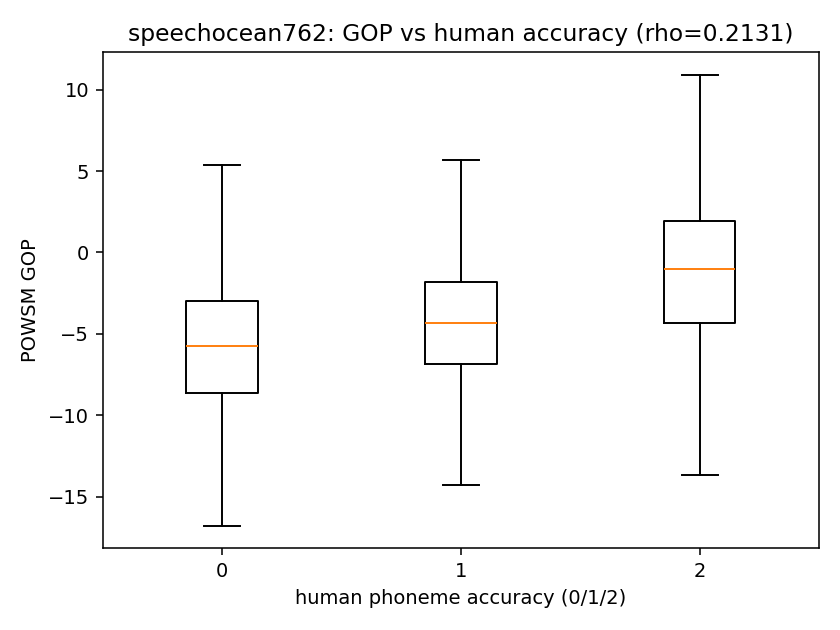
\includegraphics[width=0.62\linewidth]{gop_vs_accuracy.png}
  \end{center}
}

\block{Future Work}{
  \begin{itemize}
    \item \textbf{A perceived-annotated L2 corpus} --- the single gating resource;
      with it, this recipe scales directly.
    \item \textbf{Per-accent adapters} --- one small adapter per L1 over a frozen
      POWSM backbone.
    \item \textbf{Expert-in-the-loop data flywheel} --- the app surfaces auto-annotations
      to linguists; corrections become training data $\rightarrow$ better adapters
      (TÜBİTAK panel, in progress).
  \end{itemize}
}

\block{}{
  \small
  \textbf{github.com/umitcan07/senior} \quad\textbar\quad demo: \textbf{nounce.pro}
  \\[2mm]
  Turkish-native corpus: Öğr.\ Gör.\ Dr.\ Kardelen Kılınç, Eskişehir Tech.\ Univ.
}

\end{columns}
\end{document}
